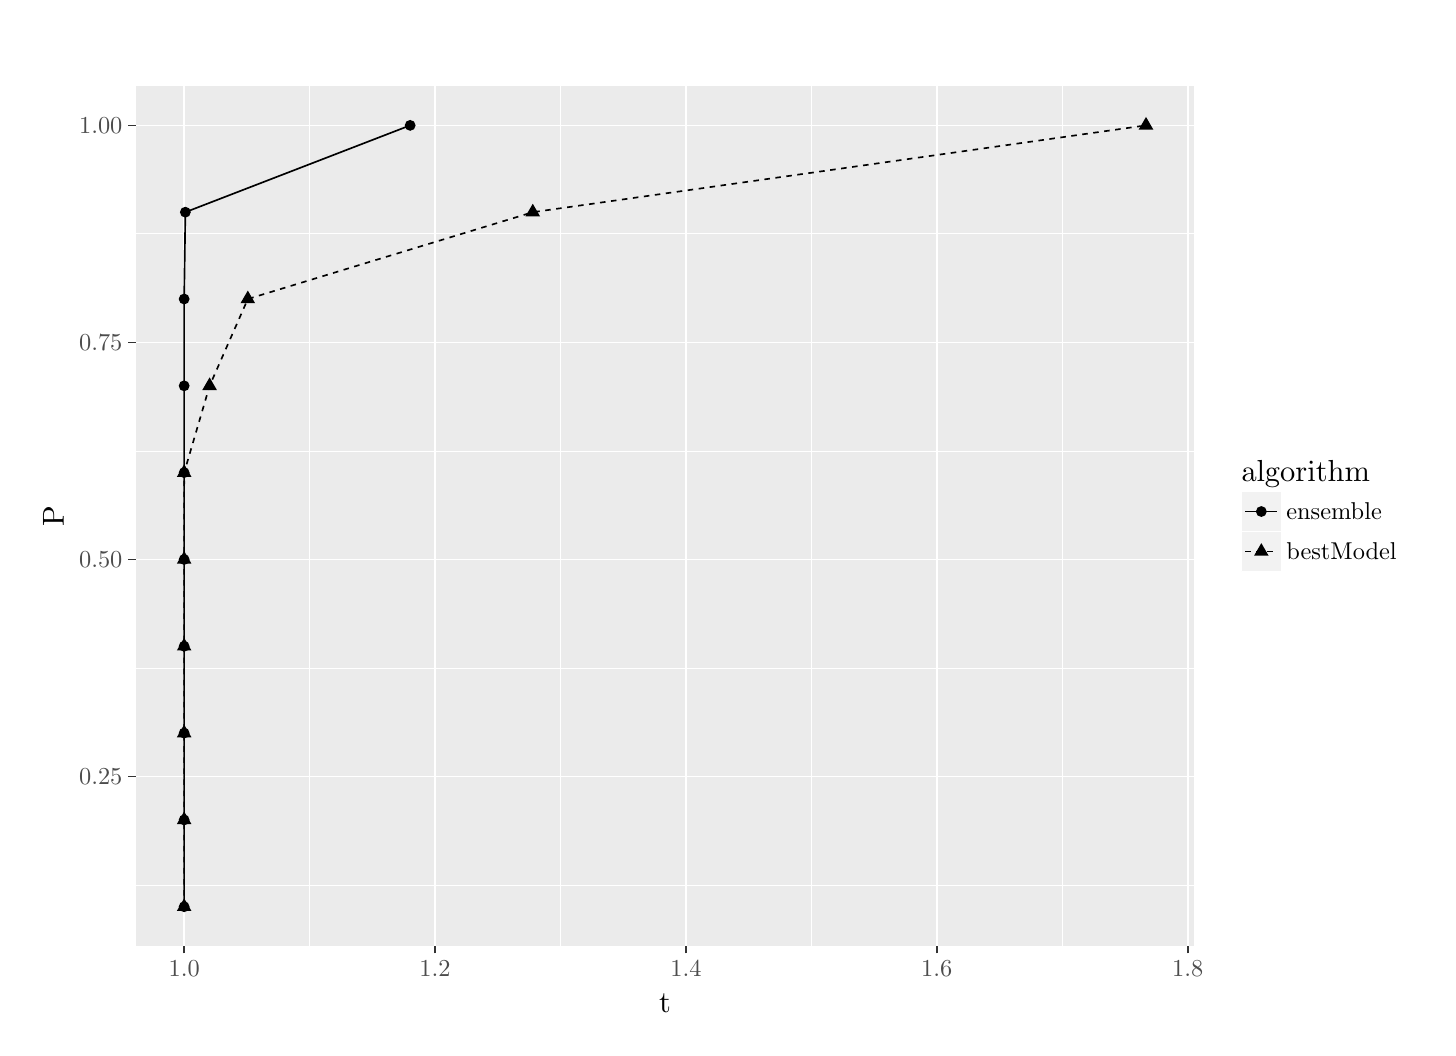
\begin{tikzpicture}[x=1pt,y=1pt]
\definecolor{fillColor}{RGB}{255,255,255}
\path[use as bounding box,fill=fillColor,fill opacity=0.00] (0,0) rectangle (505.89,361.35);
\begin{scope}
\path[clip] (  0.00,  0.00) rectangle (505.89,361.35);
\definecolor{drawColor}{RGB}{255,255,255}
\definecolor{fillColor}{RGB}{255,255,255}

\path[draw=drawColor,line width= 0.6pt,line join=round,line cap=round,fill=fillColor] (  0.00, -0.00) rectangle (505.89,361.35);
\end{scope}
\begin{scope}
\path[clip] ( 39.17, 29.59) rectangle (421.48,340.16);
\definecolor{fillColor}{gray}{0.92}

\path[fill=fillColor] ( 39.17, 29.59) rectangle (421.48,340.16);
\definecolor{drawColor}{RGB}{255,255,255}

\path[draw=drawColor,line width= 0.3pt,line join=round] ( 39.17, 51.55) --
	(421.48, 51.55);

\path[draw=drawColor,line width= 0.3pt,line join=round] ( 39.17,129.97) --
	(421.48,129.97);

\path[draw=drawColor,line width= 0.3pt,line join=round] ( 39.17,208.40) --
	(421.48,208.40);

\path[draw=drawColor,line width= 0.3pt,line join=round] ( 39.17,286.83) --
	(421.48,286.83);

\path[draw=drawColor,line width= 0.3pt,line join=round] (101.87, 29.59) --
	(101.87,340.16);

\path[draw=drawColor,line width= 0.3pt,line join=round] (192.53, 29.59) --
	(192.53,340.16);

\path[draw=drawColor,line width= 0.3pt,line join=round] (283.19, 29.59) --
	(283.19,340.16);

\path[draw=drawColor,line width= 0.3pt,line join=round] (373.84, 29.59) --
	(373.84,340.16);

\path[draw=drawColor,line width= 0.6pt,line join=round] ( 39.17, 90.76) --
	(421.48, 90.76);

\path[draw=drawColor,line width= 0.6pt,line join=round] ( 39.17,169.19) --
	(421.48,169.19);

\path[draw=drawColor,line width= 0.6pt,line join=round] ( 39.17,247.61) --
	(421.48,247.61);

\path[draw=drawColor,line width= 0.6pt,line join=round] ( 39.17,326.04) --
	(421.48,326.04);

\path[draw=drawColor,line width= 0.6pt,line join=round] ( 56.54, 29.59) --
	( 56.54,340.16);

\path[draw=drawColor,line width= 0.6pt,line join=round] (147.20, 29.59) --
	(147.20,340.16);

\path[draw=drawColor,line width= 0.6pt,line join=round] (237.86, 29.59) --
	(237.86,340.16);

\path[draw=drawColor,line width= 0.6pt,line join=round] (328.51, 29.59) --
	(328.51,340.16);

\path[draw=drawColor,line width= 0.6pt,line join=round] (419.17, 29.59) --
	(419.17,340.16);
\definecolor{drawColor}{RGB}{0,0,0}

\path[draw=drawColor,line width= 0.6pt,line join=round] ( 56.54, 43.70) --
	( 56.54, 75.07) --
	( 56.54,106.45) --
	( 56.54,137.82) --
	( 56.54,169.19) --
	( 56.54,200.56) --
	( 56.54,231.93) --
	( 56.54,263.30) --
	( 56.98,294.67) --
	(138.21,326.04);

\path[draw=drawColor,line width= 0.6pt,dash pattern=on 2pt off 2pt ,line join=round] ( 56.54, 43.70) --
	( 56.54, 75.07) --
	( 56.54,106.45) --
	( 56.54,137.82) --
	( 56.54,169.19) --
	( 56.55,200.56) --
	( 65.74,231.93) --
	( 79.55,263.30) --
	(182.52,294.67) --
	(404.11,326.04);
\definecolor{fillColor}{RGB}{0,0,0}

\path[fill=fillColor] ( 56.54, 43.70) circle (  1.96);

\path[fill=fillColor] ( 56.54, 75.07) circle (  1.96);

\path[fill=fillColor] ( 56.54,106.45) circle (  1.96);

\path[fill=fillColor] ( 56.54,137.82) circle (  1.96);

\path[fill=fillColor] ( 56.54,169.19) circle (  1.96);

\path[fill=fillColor] ( 56.54,200.56) circle (  1.96);

\path[fill=fillColor] ( 56.54,231.93) circle (  1.96);

\path[fill=fillColor] ( 56.54,263.30) circle (  1.96);

\path[fill=fillColor] ( 56.98,294.67) circle (  1.96);

\path[fill=fillColor] (138.21,326.04) circle (  1.96);

\path[fill=fillColor] ( 56.54, 46.75) --
	( 59.19, 42.18) --
	( 53.90, 42.18) --
	cycle;

\path[fill=fillColor] ( 56.54, 78.13) --
	( 59.19, 73.55) --
	( 53.90, 73.55) --
	cycle;

\path[fill=fillColor] ( 56.54,109.50) --
	( 59.19,104.92) --
	( 53.90,104.92) --
	cycle;

\path[fill=fillColor] ( 56.54,140.87) --
	( 59.19,136.29) --
	( 53.90,136.29) --
	cycle;

\path[fill=fillColor] ( 56.54,172.24) --
	( 59.19,167.66) --
	( 53.90,167.66) --
	cycle;

\path[fill=fillColor] ( 56.55,203.61) --
	( 59.19,199.03) --
	( 53.91,199.03) --
	cycle;

\path[fill=fillColor] ( 65.74,234.98) --
	( 68.38,230.40) --
	( 63.09,230.40) --
	cycle;

\path[fill=fillColor] ( 79.55,266.35) --
	( 82.19,261.77) --
	( 76.90,261.77) --
	cycle;

\path[fill=fillColor] (182.52,297.72) --
	(185.16,293.15) --
	(179.87,293.15) --
	cycle;

\path[fill=fillColor] (404.11,329.09) --
	(406.75,324.52) --
	(401.46,324.52) --
	cycle;
\end{scope}
\begin{scope}
\path[clip] (  0.00,  0.00) rectangle (505.89,361.35);
\definecolor{drawColor}{gray}{0.30}

\node[text=drawColor,anchor=base east,inner sep=0pt, outer sep=0pt, scale=  0.88] at ( 34.22, 87.73) {0.25};

\node[text=drawColor,anchor=base east,inner sep=0pt, outer sep=0pt, scale=  0.88] at ( 34.22,166.16) {0.50};

\node[text=drawColor,anchor=base east,inner sep=0pt, outer sep=0pt, scale=  0.88] at ( 34.22,244.58) {0.75};

\node[text=drawColor,anchor=base east,inner sep=0pt, outer sep=0pt, scale=  0.88] at ( 34.22,323.01) {1.00};
\end{scope}
\begin{scope}
\path[clip] (  0.00,  0.00) rectangle (505.89,361.35);
\definecolor{drawColor}{gray}{0.20}

\path[draw=drawColor,line width= 0.6pt,line join=round] ( 36.42, 90.76) --
	( 39.17, 90.76);

\path[draw=drawColor,line width= 0.6pt,line join=round] ( 36.42,169.19) --
	( 39.17,169.19);

\path[draw=drawColor,line width= 0.6pt,line join=round] ( 36.42,247.61) --
	( 39.17,247.61);

\path[draw=drawColor,line width= 0.6pt,line join=round] ( 36.42,326.04) --
	( 39.17,326.04);
\end{scope}
\begin{scope}
\path[clip] (  0.00,  0.00) rectangle (505.89,361.35);
\definecolor{drawColor}{gray}{0.20}

\path[draw=drawColor,line width= 0.6pt,line join=round] ( 56.54, 26.84) --
	( 56.54, 29.59);

\path[draw=drawColor,line width= 0.6pt,line join=round] (147.20, 26.84) --
	(147.20, 29.59);

\path[draw=drawColor,line width= 0.6pt,line join=round] (237.86, 26.84) --
	(237.86, 29.59);

\path[draw=drawColor,line width= 0.6pt,line join=round] (328.51, 26.84) --
	(328.51, 29.59);

\path[draw=drawColor,line width= 0.6pt,line join=round] (419.17, 26.84) --
	(419.17, 29.59);
\end{scope}
\begin{scope}
\path[clip] (  0.00,  0.00) rectangle (505.89,361.35);
\definecolor{drawColor}{gray}{0.30}

\node[text=drawColor,anchor=base,inner sep=0pt, outer sep=0pt, scale=  0.88] at ( 56.54, 18.58) {1.0};

\node[text=drawColor,anchor=base,inner sep=0pt, outer sep=0pt, scale=  0.88] at (147.20, 18.58) {1.2};

\node[text=drawColor,anchor=base,inner sep=0pt, outer sep=0pt, scale=  0.88] at (237.86, 18.58) {1.4};

\node[text=drawColor,anchor=base,inner sep=0pt, outer sep=0pt, scale=  0.88] at (328.51, 18.58) {1.6};

\node[text=drawColor,anchor=base,inner sep=0pt, outer sep=0pt, scale=  0.88] at (419.17, 18.58) {1.8};
\end{scope}
\begin{scope}
\path[clip] (  0.00,  0.00) rectangle (505.89,361.35);
\definecolor{drawColor}{RGB}{0,0,0}

\node[text=drawColor,anchor=base,inner sep=0pt, outer sep=0pt, scale=  1.10] at (230.32,  5.50) {t};
\end{scope}
\begin{scope}
\path[clip] (  0.00,  0.00) rectangle (505.89,361.35);
\definecolor{drawColor}{RGB}{0,0,0}

\node[text=drawColor,rotate= 90.00,anchor=base,inner sep=0pt, outer sep=0pt, scale=  1.10] at ( 13.08,184.87) {P};
\end{scope}
\begin{scope}
\path[clip] (  0.00,  0.00) rectangle (505.89,361.35);
\definecolor{fillColor}{RGB}{255,255,255}

\path[fill=fillColor] (432.86,159.13) rectangle (500.39,210.61);
\end{scope}
\begin{scope}
\path[clip] (  0.00,  0.00) rectangle (505.89,361.35);
\definecolor{drawColor}{RGB}{0,0,0}

\node[text=drawColor,anchor=base west,inner sep=0pt, outer sep=0pt, scale=  1.10] at (438.55,197.35) {algorithm};
\end{scope}
\begin{scope}
\path[clip] (  0.00,  0.00) rectangle (505.89,361.35);
\definecolor{drawColor}{RGB}{255,255,255}
\definecolor{fillColor}{gray}{0.95}

\path[draw=drawColor,line width= 0.6pt,line join=round,line cap=round,fill=fillColor] (438.55,179.28) rectangle (453.01,193.73);
\end{scope}
\begin{scope}
\path[clip] (  0.00,  0.00) rectangle (505.89,361.35);
\definecolor{drawColor}{RGB}{0,0,0}

\path[draw=drawColor,line width= 0.6pt,line join=round] (440.00,186.51) -- (451.56,186.51);
\end{scope}
\begin{scope}
\path[clip] (  0.00,  0.00) rectangle (505.89,361.35);
\definecolor{fillColor}{RGB}{0,0,0}

\path[fill=fillColor] (445.78,186.51) circle (  1.96);
\end{scope}
\begin{scope}
\path[clip] (  0.00,  0.00) rectangle (505.89,361.35);
\definecolor{drawColor}{RGB}{255,255,255}
\definecolor{fillColor}{gray}{0.95}

\path[draw=drawColor,line width= 0.6pt,line join=round,line cap=round,fill=fillColor] (438.55,164.82) rectangle (453.01,179.28);
\end{scope}
\begin{scope}
\path[clip] (  0.00,  0.00) rectangle (505.89,361.35);
\definecolor{drawColor}{RGB}{0,0,0}

\path[draw=drawColor,line width= 0.6pt,dash pattern=on 2pt off 2pt ,line join=round] (440.00,172.05) -- (451.56,172.05);
\end{scope}
\begin{scope}
\path[clip] (  0.00,  0.00) rectangle (505.89,361.35);
\definecolor{fillColor}{RGB}{0,0,0}

\path[fill=fillColor] (445.78,175.10) --
	(448.42,170.53) --
	(443.14,170.53) --
	cycle;
\end{scope}
\begin{scope}
\path[clip] (  0.00,  0.00) rectangle (505.89,361.35);
\definecolor{drawColor}{RGB}{0,0,0}

\node[text=drawColor,anchor=base west,inner sep=0pt, outer sep=0pt, scale=  0.88] at (454.82,183.47) {ensemble};
\end{scope}
\begin{scope}
\path[clip] (  0.00,  0.00) rectangle (505.89,361.35);
\definecolor{drawColor}{RGB}{0,0,0}

\node[text=drawColor,anchor=base west,inner sep=0pt, outer sep=0pt, scale=  0.88] at (454.82,169.02) {bestModel};
\end{scope}
\end{tikzpicture}

